\documentclass[twoside]{article}

% Packages required by doxygen
\usepackage{fixltx2e}
\usepackage{calc}
\usepackage{doxygen}
\usepackage[export]{adjustbox} % also loads graphicx
\usepackage{graphicx}
\usepackage[utf8]{inputenc}
\usepackage{makeidx}
\usepackage{multicol}
\usepackage{multirow}
\PassOptionsToPackage{warn}{textcomp}
\usepackage{textcomp}
\usepackage[nointegrals]{wasysym}
\usepackage[table]{xcolor}

% NLS support packages
\usepackage[T2A]{fontenc}
\usepackage[russian]{babel}

% Font selection
\usepackage[T1]{fontenc}
\usepackage[scaled=.90]{helvet}
\usepackage{courier}
\usepackage{amssymb}
\usepackage{sectsty}
\renewcommand{\familydefault}{\sfdefault}
\allsectionsfont{%
  \fontseries{bc}\selectfont%
  \color{darkgray}%
}
\renewcommand{\DoxyLabelFont}{%
  \fontseries{bc}\selectfont%
  \color{darkgray}%
}
\newcommand{\+}{\discretionary{\mbox{\scriptsize$\hookleftarrow$}}{}{}}

% Page & text layout
\usepackage{geometry}
\geometry{%
  a4paper,%
  top=2.5cm,%
  bottom=2.5cm,%
  left=2.5cm,%
  right=2.5cm%
}
\tolerance=750
\hfuzz=15pt
\hbadness=750
\setlength{\emergencystretch}{15pt}
\setlength{\parindent}{0cm}
\setlength{\parskip}{0.2cm}
\makeatletter
\renewcommand{\paragraph}{%
  \@startsection{paragraph}{4}{0ex}{-1.0ex}{1.0ex}{%
    \normalfont\normalsize\bfseries\SS@parafont%
  }%
}
\renewcommand{\subparagraph}{%
  \@startsection{subparagraph}{5}{0ex}{-1.0ex}{1.0ex}{%
    \normalfont\normalsize\bfseries\SS@subparafont%
  }%
}
\makeatother

% Headers & footers
\usepackage{fancyhdr}
\pagestyle{fancyplain}
\fancyhead[LE]{\fancyplain{}{\bfseries\thepage}}
\fancyhead[CE]{\fancyplain{}{}}
\fancyhead[RE]{\fancyplain{}{\bfseries\leftmark}}
\fancyhead[LO]{\fancyplain{}{\bfseries\rightmark}}
\fancyhead[CO]{\fancyplain{}{}}
\fancyhead[RO]{\fancyplain{}{\bfseries\thepage}}
\fancyfoot[LE]{\fancyplain{}{}}
\fancyfoot[CE]{\fancyplain{}{}}
\fancyfoot[RE]{\fancyplain{}{\bfseries\scriptsize Документация по КДЗ модуль 3. }}
\fancyfoot[LO]{\fancyplain{}{\bfseries\scriptsize Документация по КДЗ модуль 3. }}
\fancyfoot[CO]{\fancyplain{}{}}
\fancyfoot[RO]{\fancyplain{}{}}
\renewcommand{\footrulewidth}{0.4pt}
\renewcommand{\sectionmark}[1]{%
  \markright{\thesection\ #1}%
}

% Indices & bibliography
\usepackage{natbib}
\usepackage[titles]{tocloft}
\setcounter{tocdepth}{3}
\setcounter{secnumdepth}{5}
\makeindex

% Custom commands
\newcommand{\clearemptydoublepage}{%
  \newpage{\pagestyle{empty}\cleardoublepage}%
}

% Custom packages
\usepackage{pdfpages}


%===== C O N T E N T S =====

\begin{document}

% Titlepage & ToC
\pagenumbering{roman}
\begin{titlepage}
\begin{center}
\vspace*{1cm}
{\large НАЦИОНАЛЬНЫЙ ИССЛЕДОВАТЕЛЬСКИЙ УНИВЕРСИТЕТ \\
«ВЫСШАЯ ШКОЛА ЭКОНОМИКИ» }\\
\vspace*{0.5cm}
{\large Факультет компьютерных наук }\\
\vspace*{0.5cm}
{\small Департамент программнoй инженерии \\
}
\vfill % заполняет длину страницы вертикально
{\large\textbf{
Контрольное домашнее задание \\
по дисциплине\\
«Программирование» \\
}}
\bigskip
{\large Тема работы: Обработка данных из файла }\\
\vfill
\begin{flushright}
Выполнил студент группы БПИ 151 \\
Абрамов А.M. \\
Преподаватель: Подбельский Вадим Валериевич \\
\end{flushright}
\vfill
Москва \number\year \\
Модуль 3
\end{center}
\end{titlepage}

\tableofcontents
\pagenumbering{arabic}

% --- add my custom headers ---
\section{Условие задачи}

\begin{DoxyImageNoCaption}
  \mbox{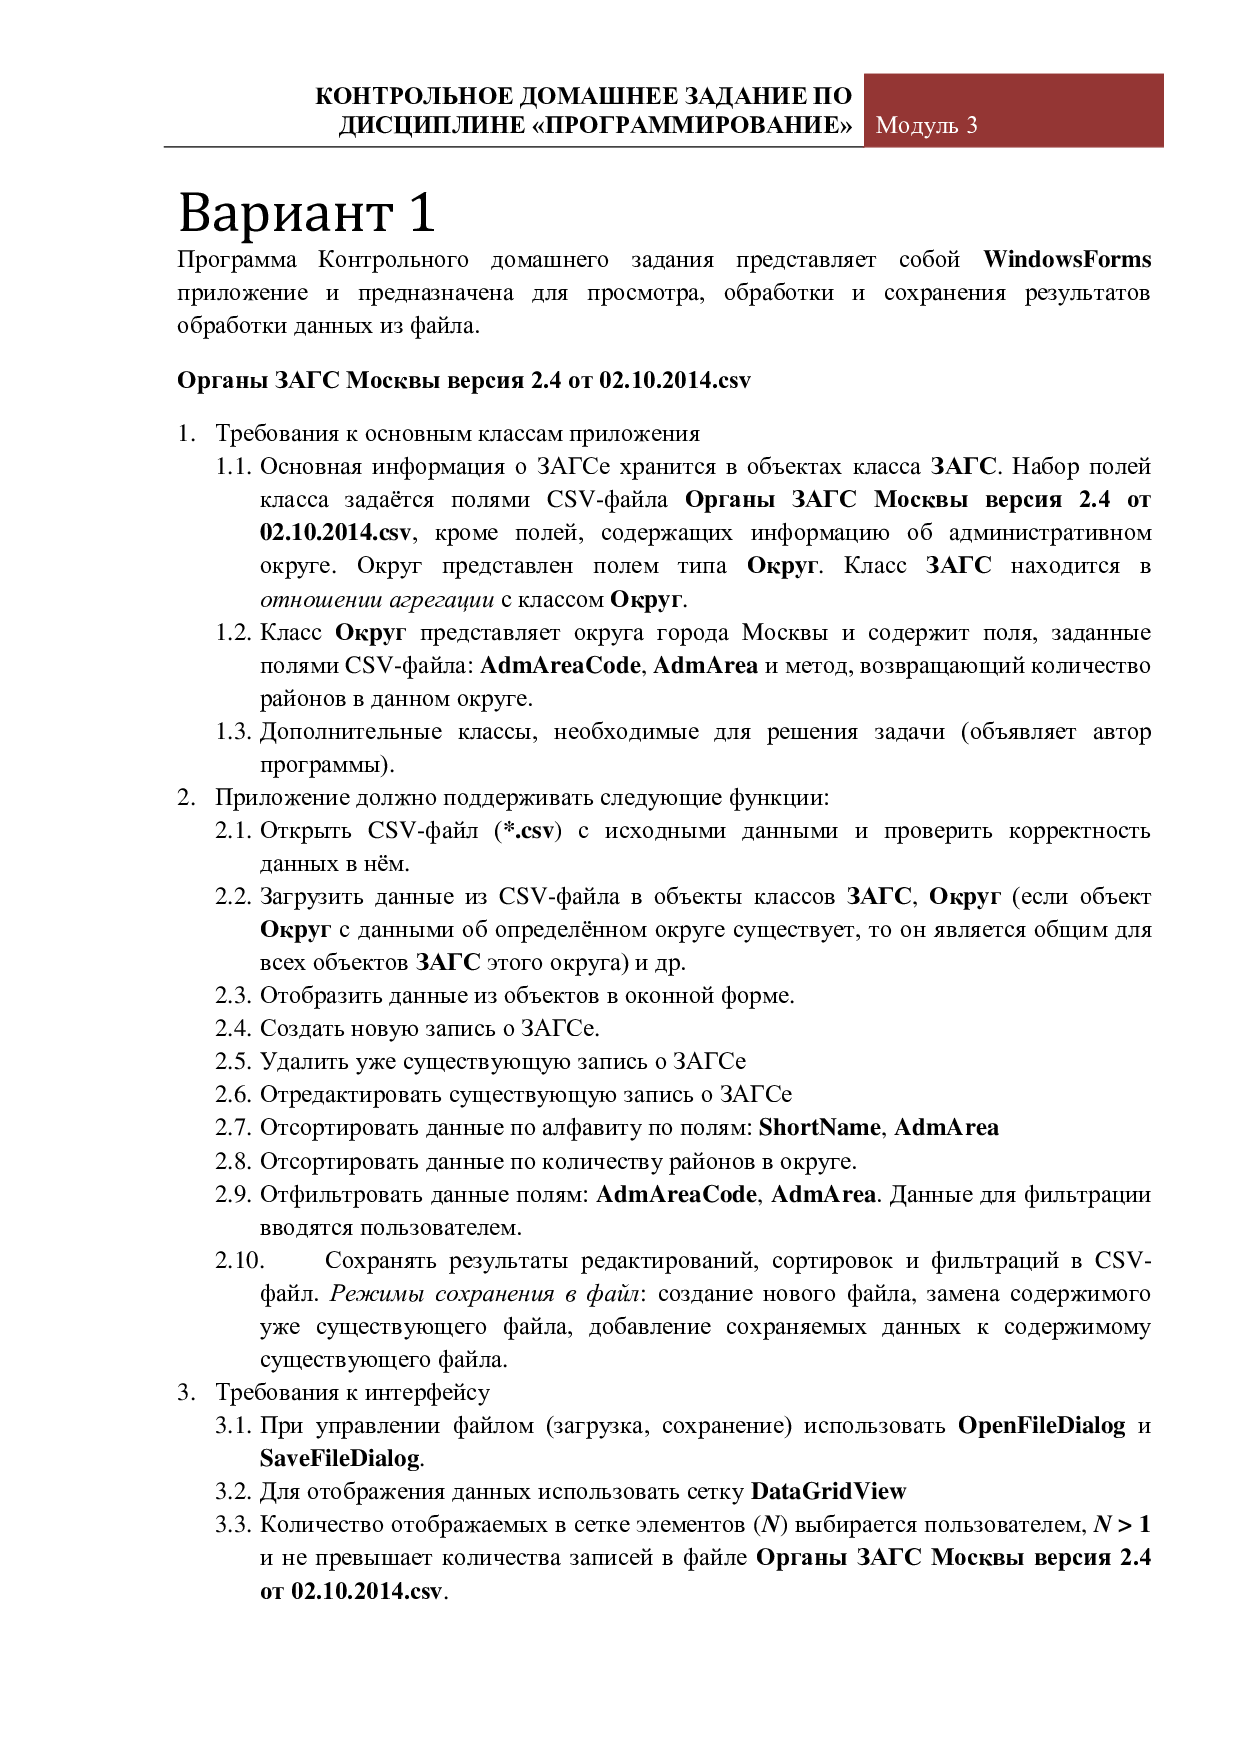
\includegraphics[height=22cm]{task_one.png}}
\end{DoxyImageNoCaption}
\newpage
\begin{DoxyImageNoCaption}
  \mbox{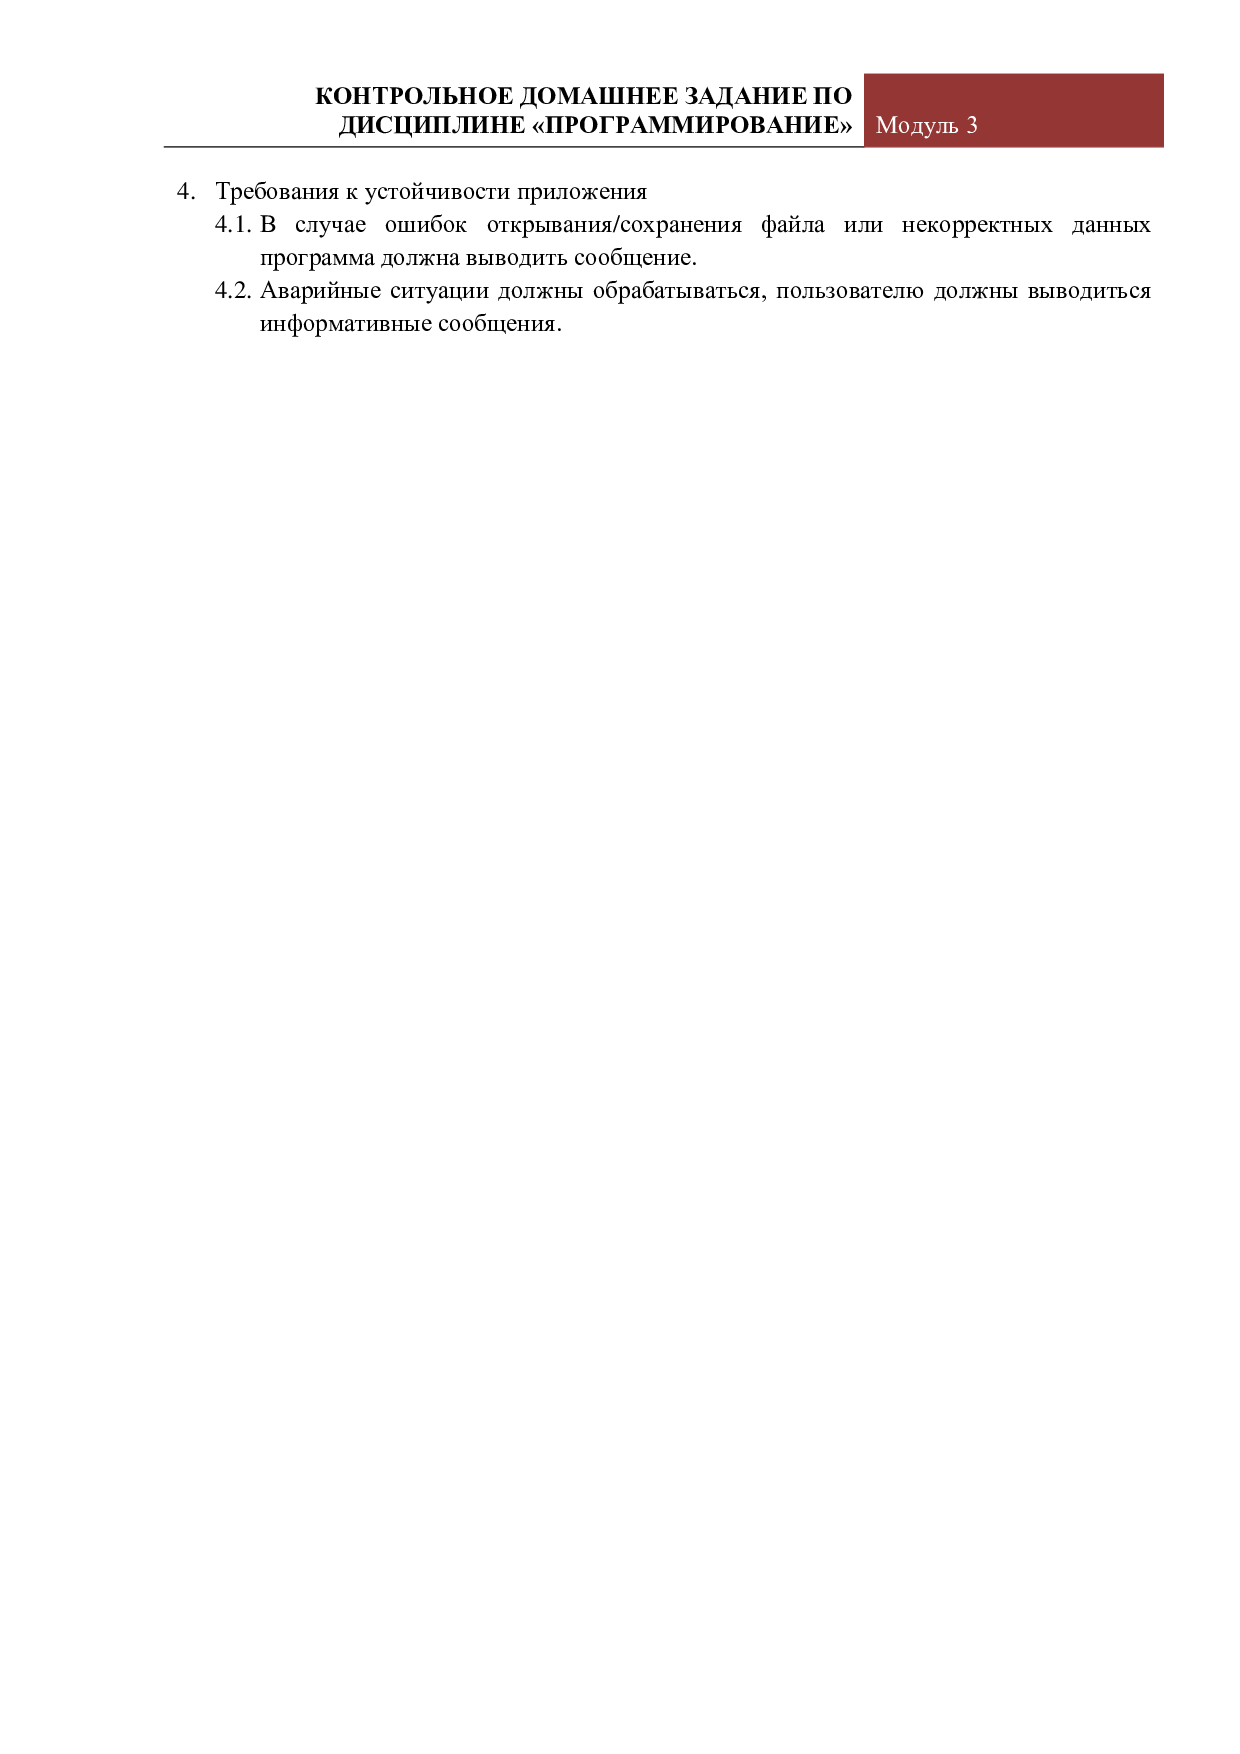
\includegraphics[height=22cm]{task_two.png}}
\end{DoxyImageNoCaption}
\newpage



\section{Функционал приложения}
\subsubsection*{Варианты использования}

Приложение позволяет просматривать C\+S\+V файлы. Просмотр данных из C\+S\+V файлов. Анализ частоты встречаемости данных. Поиск по базе данных записанной в формате C\+S\+V.

\subsubsection*{Описание интерфейса пользователя}

В программе присутствует стандартная верхняя панель меню и стандартная панель инструментов для работы с файлами. Для фильтрации данных в файле используются поля ввода расположенные над Data\+Grid\+View в котором отображаются данные из файла.

Для загрузки данных используется либо меню File, либо операцию Open на панели инструментов. Есть поддержка недавно открытых файлов. Также программа умеет запоминать последнюю посещенную директорию.

Сортировка колонок производится посредством щелканья на имени колонки. Фильтрация колонок производится посредством ввода значения для фильтра (то что должно совпадать). При поиске введенный регистр всегда учитывается. Также пользователь может воспользоваться продвинутым фильтром для более точной фильтрации.

Внизу программы представлен статус по данной таблице и по результатам фильтрации.

Также имеется поддержка для показа огранниченного набора строк и перелистывания страниц. Текущая страница и колличество строк на странице отображаются в вверху и слева от таблицы.

![alt text][interface\+\_\+menu] 
\section{Структура приложения}
![alt text][class\+\_\+diagram] 

%--- Begin generated contents ---
